\documentclass[tikz,border=3.14pt]{standalone}
\usepackage{amsmath}
\usepackage{caption}
\usetikzlibrary{3d,decorations.text,shapes.arrows,positioning,fit,backgrounds,arrows}

\begin{document}

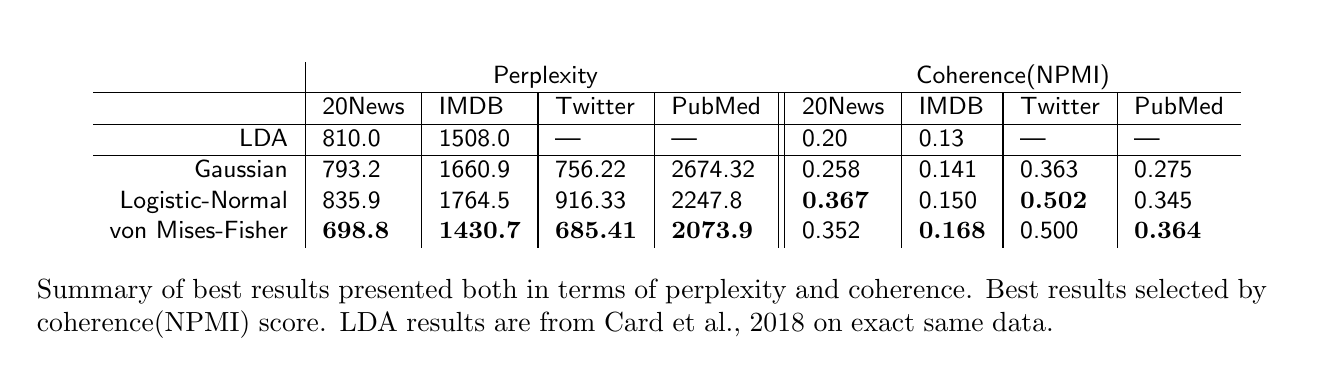
\begin{tikzpicture}[font=\sffamily\small,scale=2]

\node[text width=16cm] at (0,0) {
  \begin{table}[]
    \begin{center}
  \begin{tabular}{r|l|l|l|l||l|l|l|l}
    & \multicolumn{4}{c}{Perplexity} & \multicolumn{4}{c}{Coherence(NPMI)} \\
    \hline 
    & 20News & IMDB & Twitter & PubMed & 20News & IMDB & Twitter & PubMed \\
    \hline
    LDA & 810.0 & 1508.0 & --- & --- & 0.20 & 0.13 & --- & --- \\
    \hline
    Gaussian &   793.2 &  1660.9  &  756.22 &  2674.32  & 0.258 & 0.141 & 0.363 & 0.275  \\
    Logistic-Normal &   835.9 &  1764.5  &  916.33 &   2247.8 & {\bf 0.367} & 0.150 & {\bf 0.502}  &  0.345 \\
    von Mises-Fisher  &   {\bf 698.8} &  {\bf 1430.7}  &  {\bf 685.41}  &  {\bf 2073.9} & 0.352 & {\bf 0.168} & 0.500 & {\bf 0.364}
  \end{tabular}
  \end{center}
    \caption*{Summary of best results
      presented both in terms of perplexity and coherence. Best results selected by coherence(NPMI) score.
      LDA results are from Card et al., 2018 on exact same data.}
\end{table}};


\end{tikzpicture}
\end{document}
